\documentclass[../Article_Model_Parameters.tex]{subfiles}
\graphicspath{{\subfix{../Figures/}}}
\begin{document}
	
	\label{CH: Results}

    The parameter estimation problem was solved by fitting the process model to the dataset given in the Figure \ref{fig: estimation_results}. Each time-series present was fitted to the model separately. The blue dots indicate the data point obtained as a measurement from the laboratory experiments. The black curve represents the yield curve obtained from the initial guess of the parameters. The red curve correspond to yield curve obtained as a solution of the optimization problem. Every sub-figure is made of two figure of which one represent the cumulative yield, and the second one shows the derivative of the cumulative yield. As explained in the Chapter \ref{CH: Parameter_estimation}, the derivatives of the cumulative measurements are independent on the previous measurement and should be used for the parameter estimation.
    The parameters obtained from solving the optimization problem can be found in Table \ref{tab: Estimation_results}.
    
    \begin{figure*}[!h]
    	\centering
    	\begin{subfigure}[b]{\columnwidth}
    		\centering
    		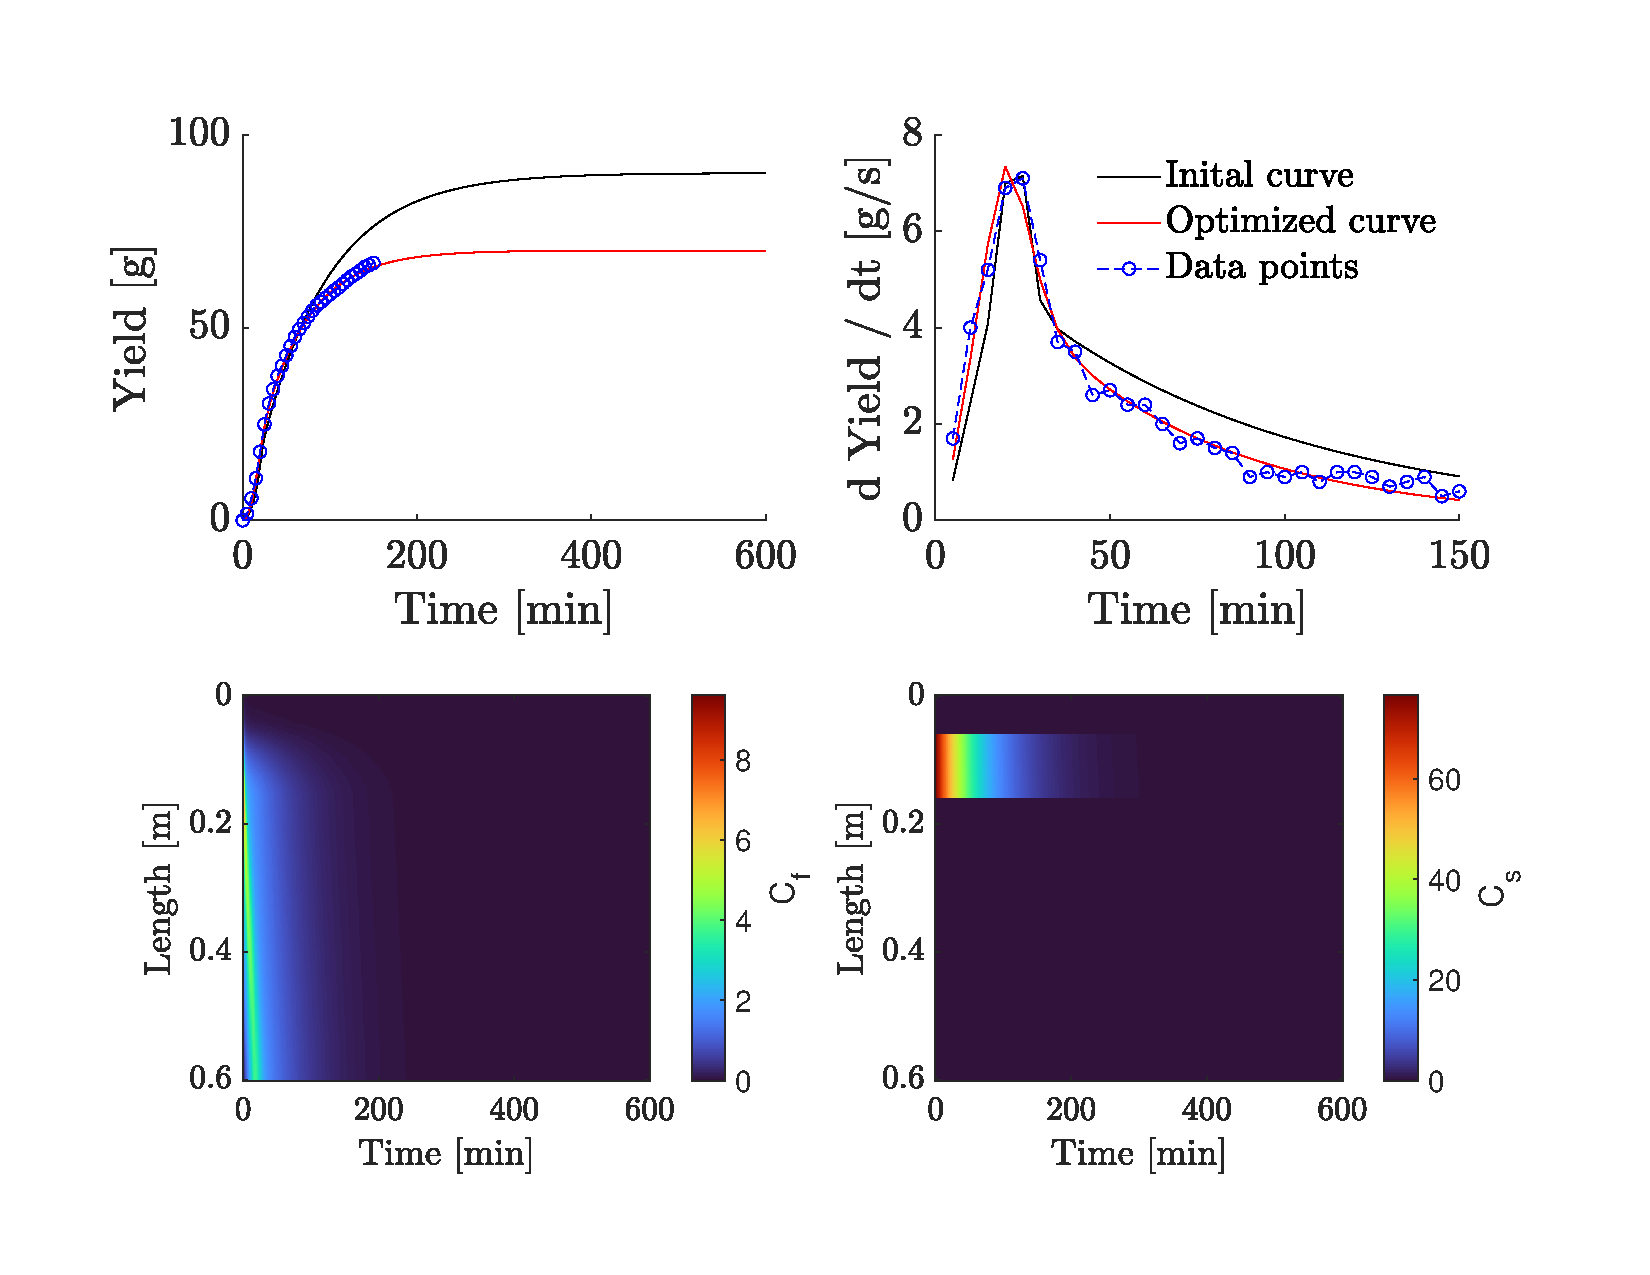
\includegraphics[trim = 2cm 10.5cm 2.5cm 2.02cm,clip,width=\textwidth]{/Results_estimation/Fitting_LUKE_T40_P200.pdf}
    		\caption{Experiment at $40^\circ C$ and $200$ bar}
    	\end{subfigure}
    	\begin{subfigure}[b]{\columnwidth}
    		\centering
    		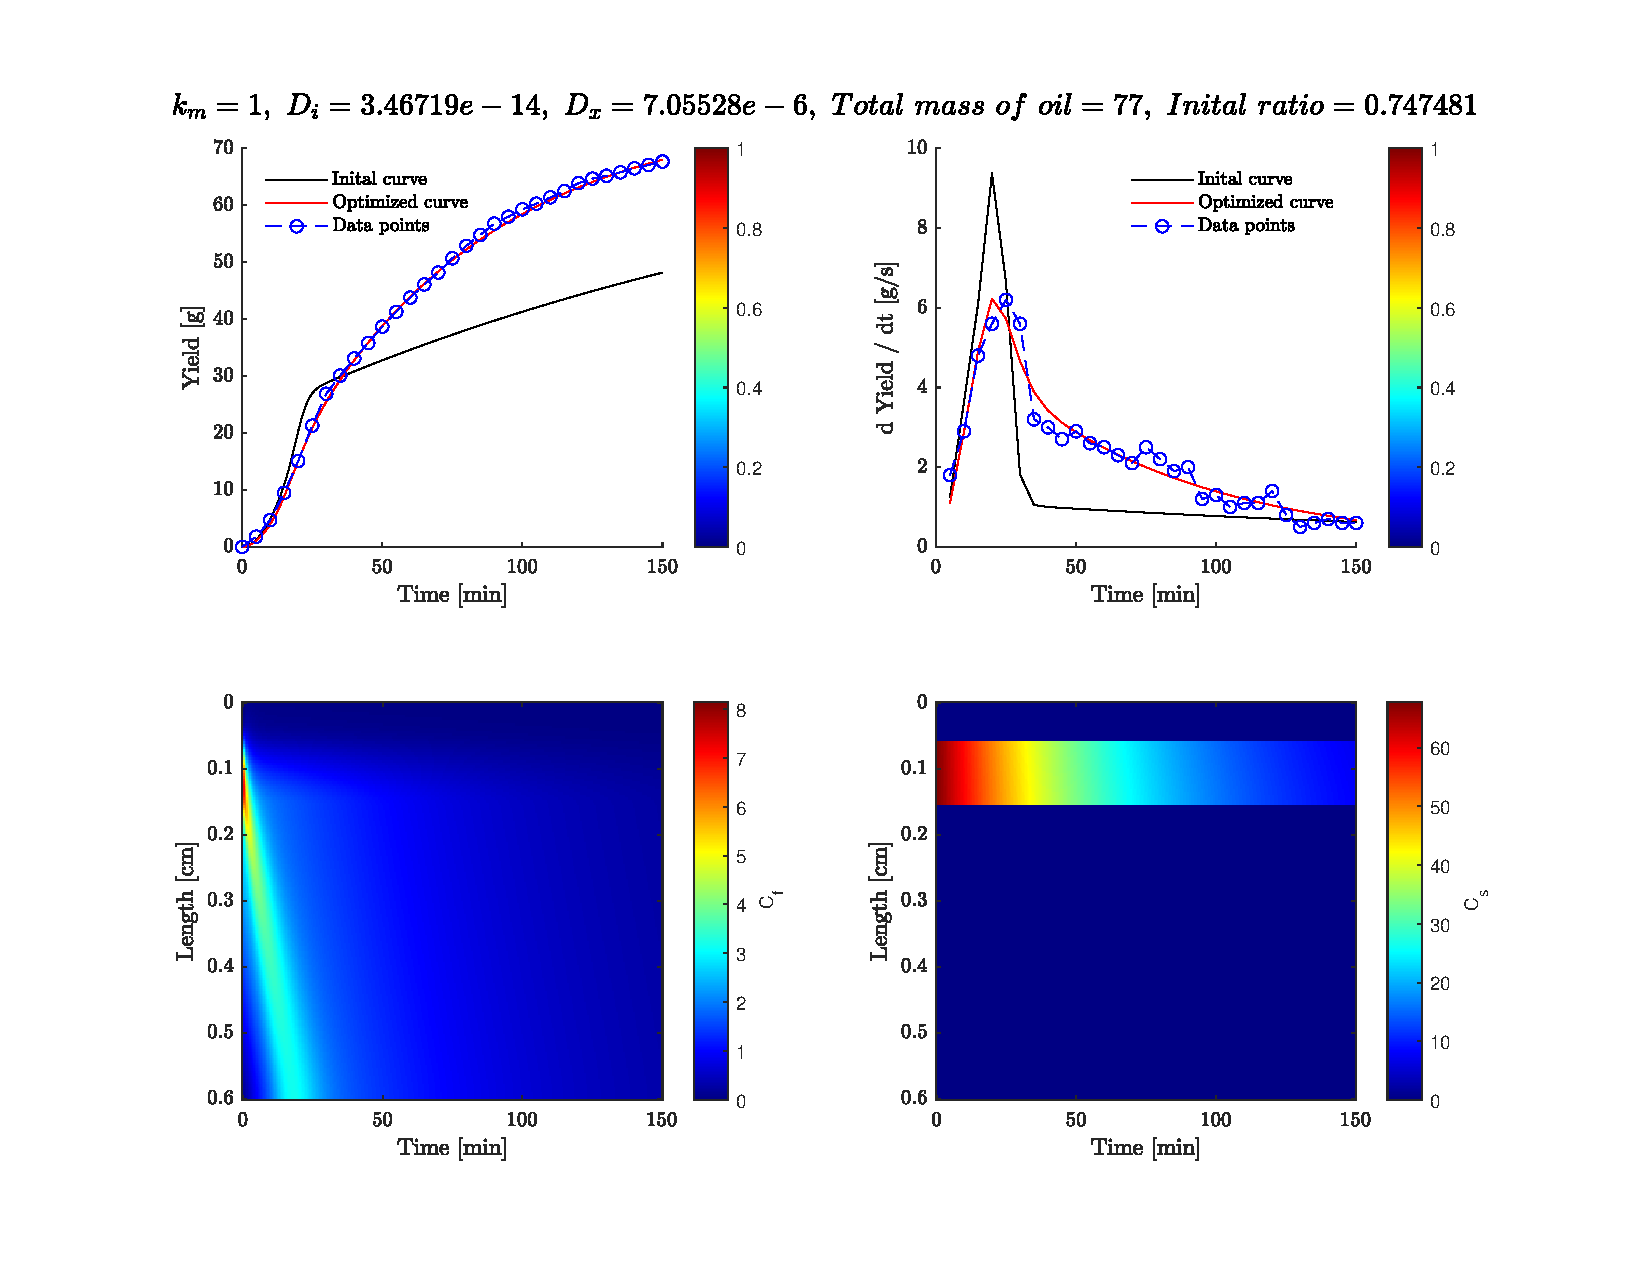
\includegraphics[trim = 2cm 10.5cm 2.5cm 2.02cm,clip,width=\textwidth]{/Results_estimation/Fitting_LUKE_T50_P200.pdf}
    		\caption{Experiment at $50^\circ C$ and $200$ bar}
    	\end{subfigure}
    	\hfill
    	\begin{subfigure}[b]{\columnwidth}
    		\centering
    		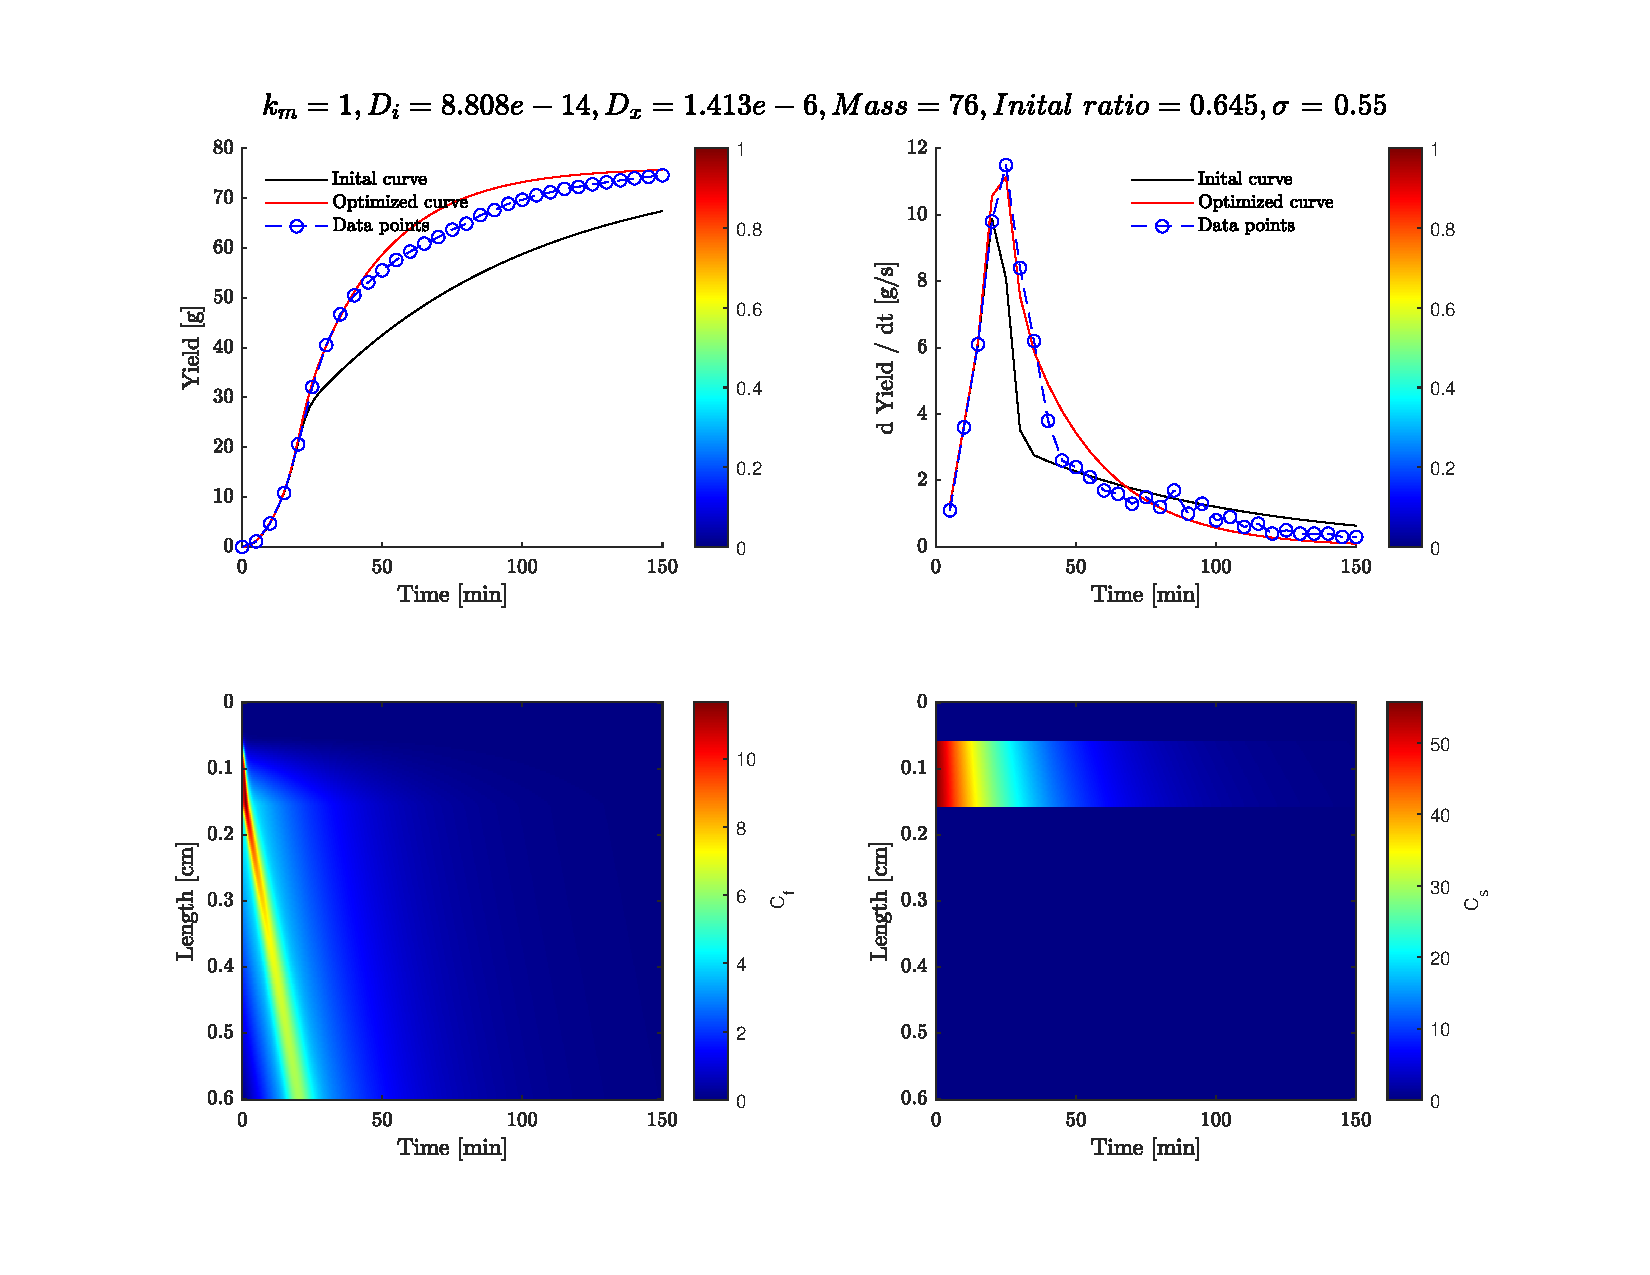
\includegraphics[trim = 2cm 10.5cm 2.5cm 2.02cm,clip,width=\textwidth]{/Results_estimation/Fitting_LUKE_T40_P300_org.pdf}
    		\caption{Experiment at $40^\circ C$ and $300$ bar}
    	\end{subfigure}
    	\begin{subfigure}[b]{\columnwidth}
    		\centering
    		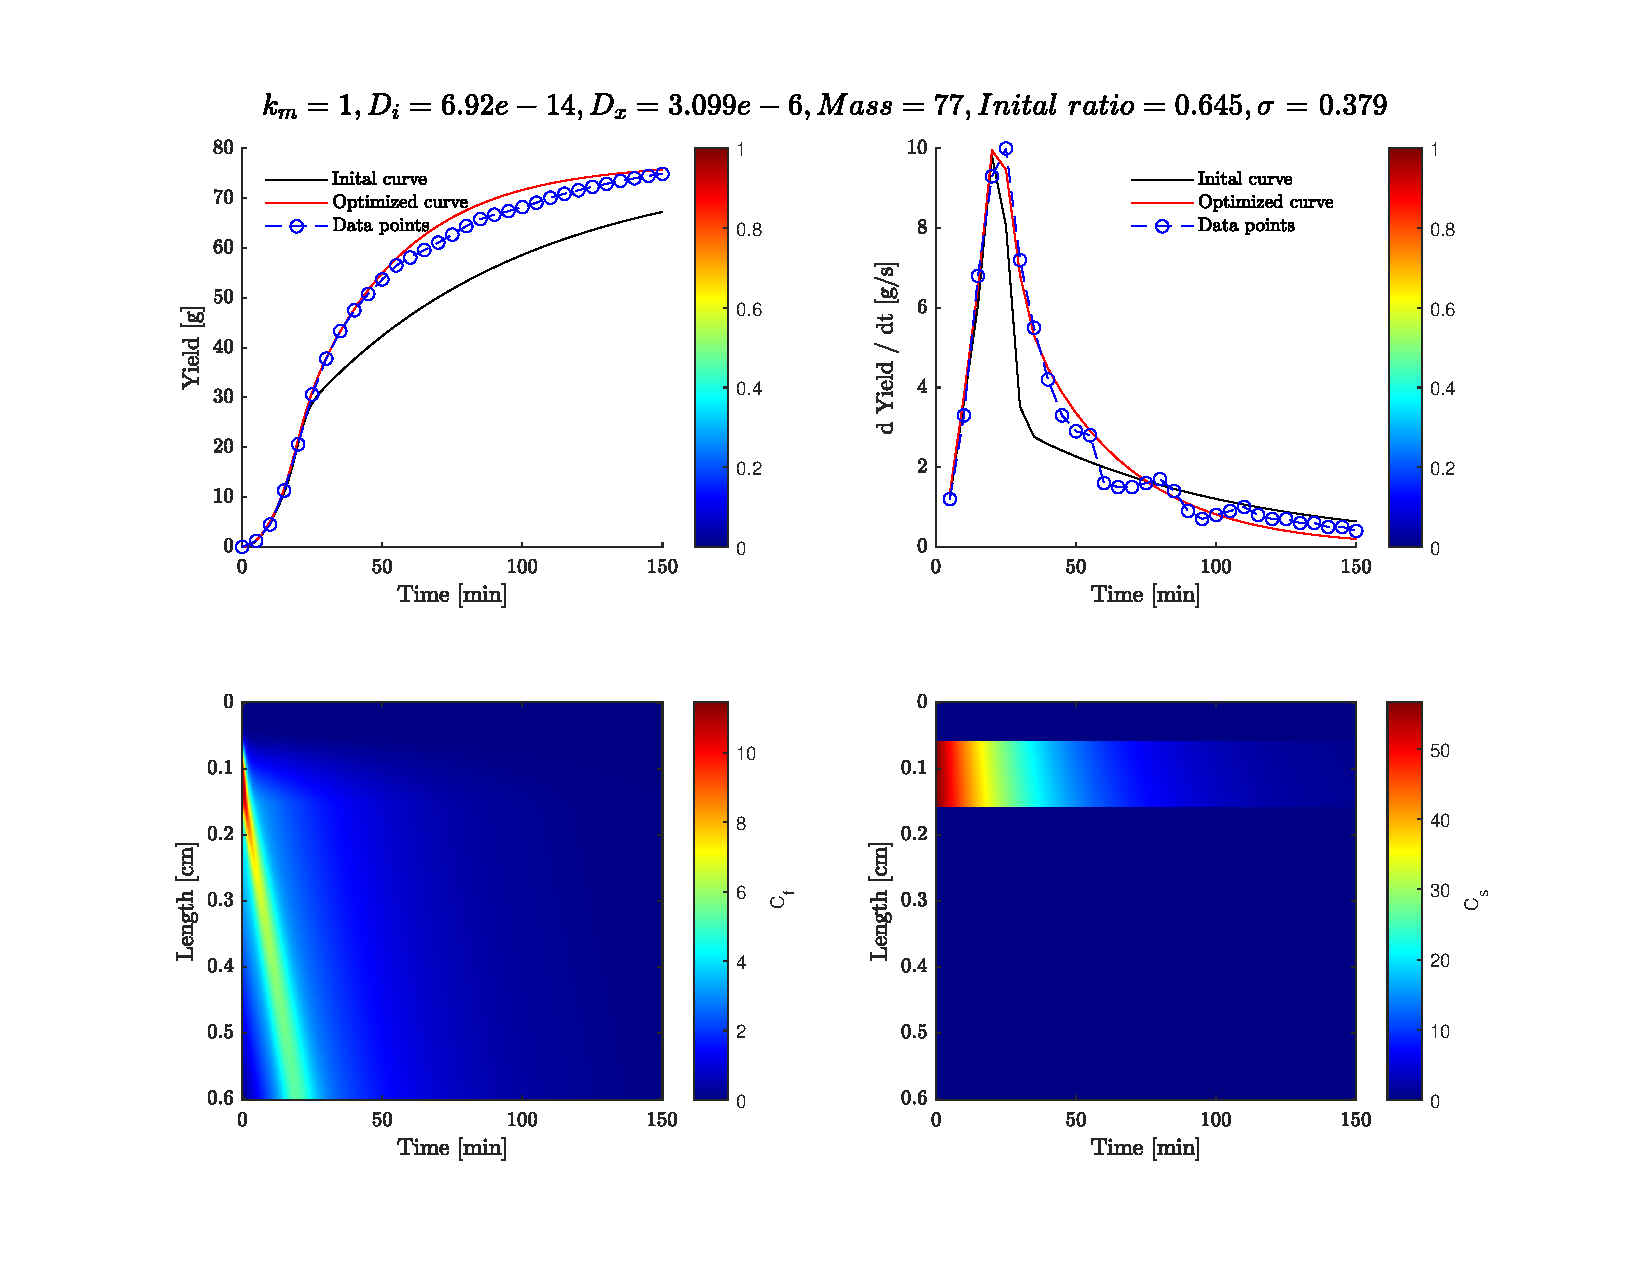
\includegraphics[trim = 2cm 10.5cm 2.5cm 2.02cm,clip,width=\textwidth]{/Results_estimation/Fitting_LUKE_T50_P300_org.pdf}
    		\caption{Experiment at $50^\circ C$ and $300$ bar}
    	\end{subfigure}
    	\caption{Results of parameter estimation}
    	\label{fig: estimation_results}
    \end{figure*}

	 %and the concentration profiles, which correspond for the optimized solution for each experiments, are presented on Figure \ref{fig: estimation_results_profiles} in Appendix \ref{CH: Profiles}.
	
	\begin{table}[!h]
		\centering
		\adjustbox{max width=\columnwidth}{%
			\csvautobooktabular{Figures/Results_estimation/estimation_2.csv} }
		\caption{Parameter estimation results rounded to fifth decimal place}
		\label{tab: Estimation_results}
	\end{table}
	
	As shown in the Table \ref{tab: Estimation_results}, the optimizer found optimal values of the partition factors ${\color{orange}k_m}$ at relatively high levels. Such a behaviour suggest that the solvent is far from the saturation, and the model can be simplified. The model reduction can be introduced by considering the limit of the concentration gradient
	
	{\footnotesize
	\begin{equation*}
		\begin{split}
			&\lim_{k_m \rightarrow \infty} \left({\color{blue}{\color{blue} c_s} }(t,z)  - \cfrac{{\color{magenta}\rho_s}}{{\color{orange}k_m}({\color{blue}T}(t,z)){\color{orange}\rho}({\color{blue}T}(t,z),{\color{red}P}(t))}  {\color{blue}c_f}(t,z) \right)  = \\
			&= \left({\color{blue}{\color{blue} c_s} }(t,z)  - \cfrac{{\color{magenta}\rho_s}}{\infty{\color{orange}\rho}({\color{blue}T}(t,z),{\color{red}P}(t))}  {\color{blue}c_f}(t,z) \right) = \left({\color{blue}{\color{blue} c_s} }(t,z) - 0 \right)
		\end{split}
	\end{equation*} }
		
	Values of the internal diffusion coefficients are distinguished for each experiment. The order of magnitude of ${\color{orange}D_i^R}$ obtained from the optimization is similar to values found by other researchers. \citet{Reverchon1996} performed the parameter estimation for the extraction process of sage oil from seeds and reported ${\color{magenta}D_i^R} \approx 6\times 10^{-13}[m^2/s]$. Figure \ref{fig: results_DI} represent the ${\color{orange}D_i^R}$ as the function of density. As the internal diffusion coefficient describes the diffusion inside of a particle, it is independent of external factors such as a fluid velocity around that particle. In such a case, the internal diffusion depends only on local conditions given by temperature and pressure, which defines the physical properties of a stagnant fluid inside of pores of a particle—considering that the internal diffusion can be represented as a function of the density of the fluid, which is uniquely defined at a given temperature and pressure in the one-phase region. The linear trend in Figure \ref{fig: results_DI} suggests that ${\color{orange}D_i^R}$ increases with fluid density.
	
	Similarly to the internal diffusion coefficient, the obtained values ${\color{orange}\Upsilon}$ can be represented as a function of the local operating conditions, or by uniquely defined physical properties such as density. Figure \ref{fig: results_upsilon} shows that of ${\color{orange}\Upsilon}$ grows with density. This can be explained if the solubility increases as the density grows. \citet{Shojaie2010}, showed that the solubility of carvone (one of the main components of caraway oil) rises together with pressure increase and decreases when temperature increases.
	
	The Figure \ref{fig:Di_upsilon_res} shows how the internal diffusivity ${\color{orange}D_i}$ (Equation \ref{EQ: C_sat_function}) as a function of the solute concentration in the solid phase at different operating conditions. The higher the density, the higher solubility according to \citet{Shojaie2010}, which results in higher values of the internal diffusion coefficient and larger curvature of ${\color{orange}D_i}$ function.

		\begin{figure}[!h]
		\centering
		\begin{subfigure}[b]{0.49\columnwidth}
			\centering
			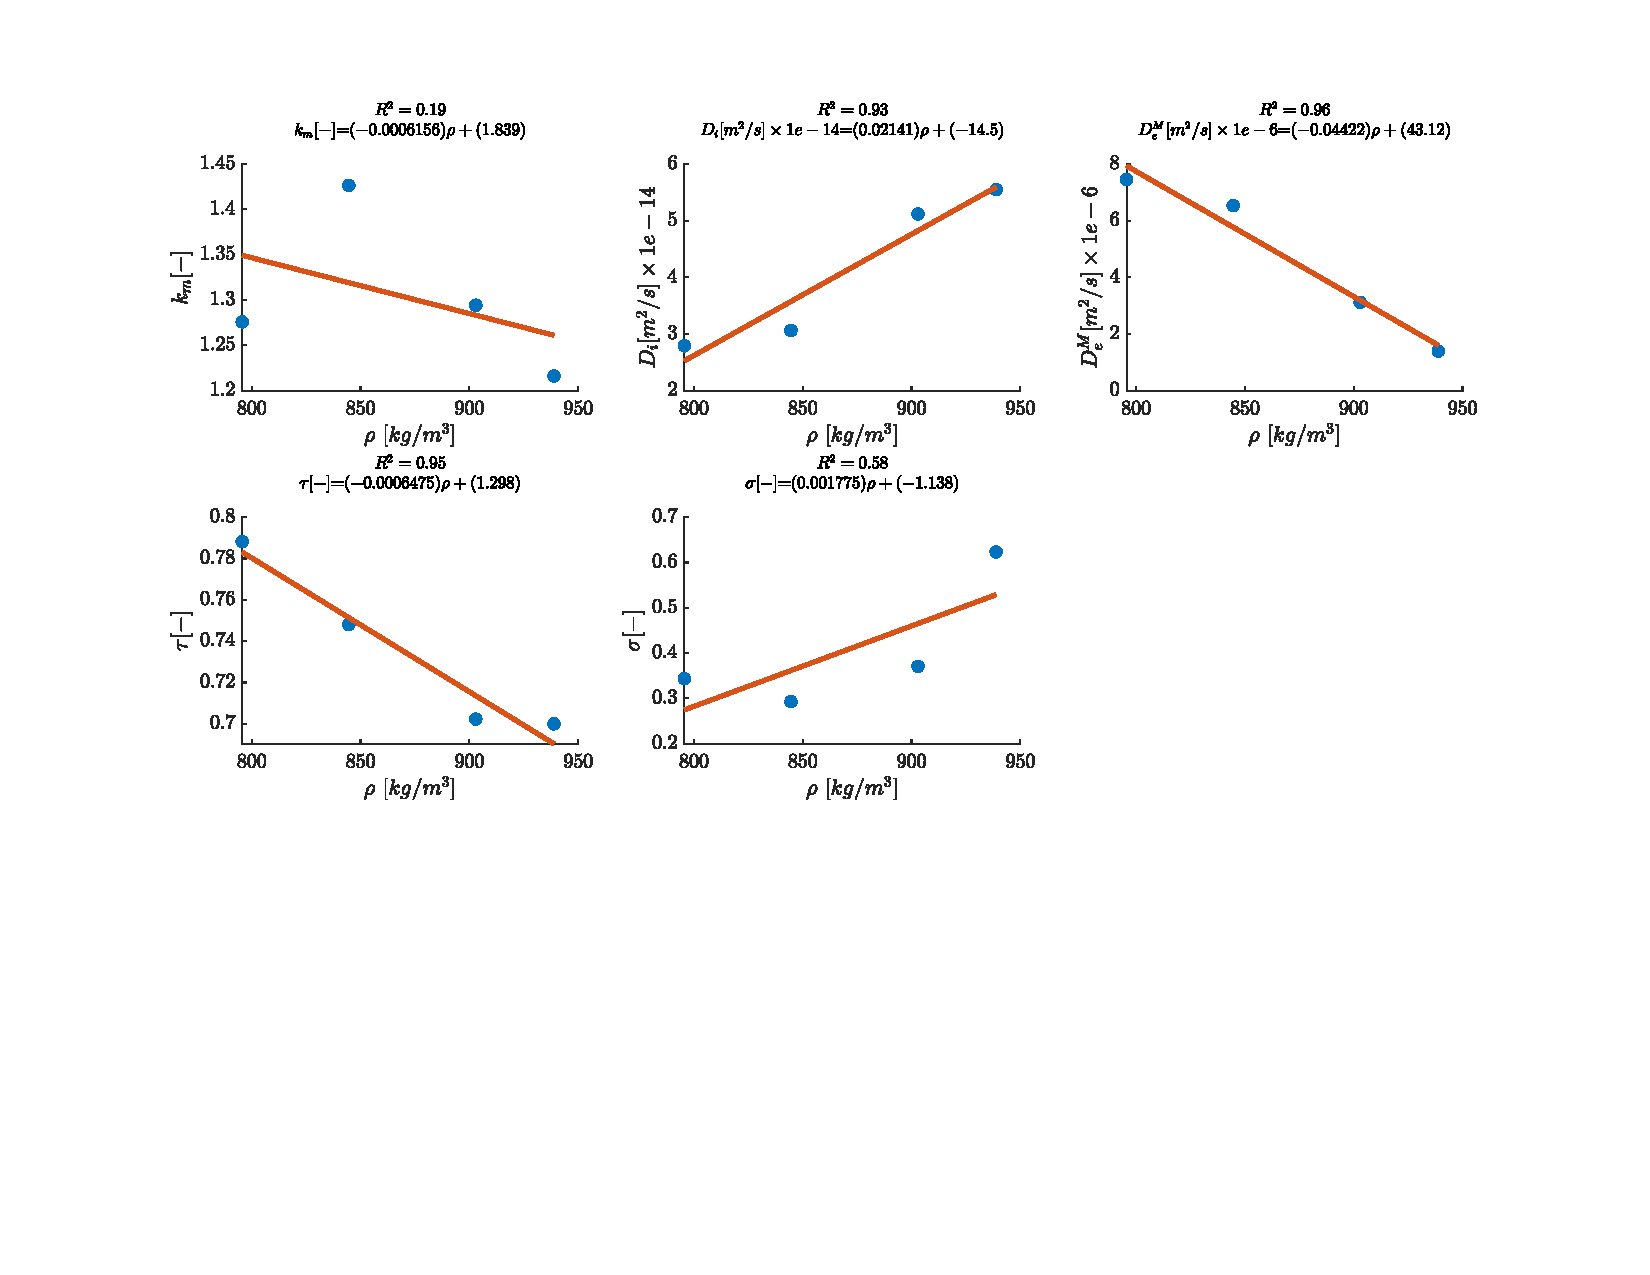
\includegraphics[trim = 10.5cm 14cm 10cm 1.5cm,clip,width=\columnwidth]{/Results_estimation/Trend_Lines_order_1.pdf}
			\caption{Dependency of ${\color{orange}D_i}$}
			\label{fig: results_DI}
		\end{subfigure}
		\begin{subfigure}[b]{0.49\columnwidth}
			\centering
			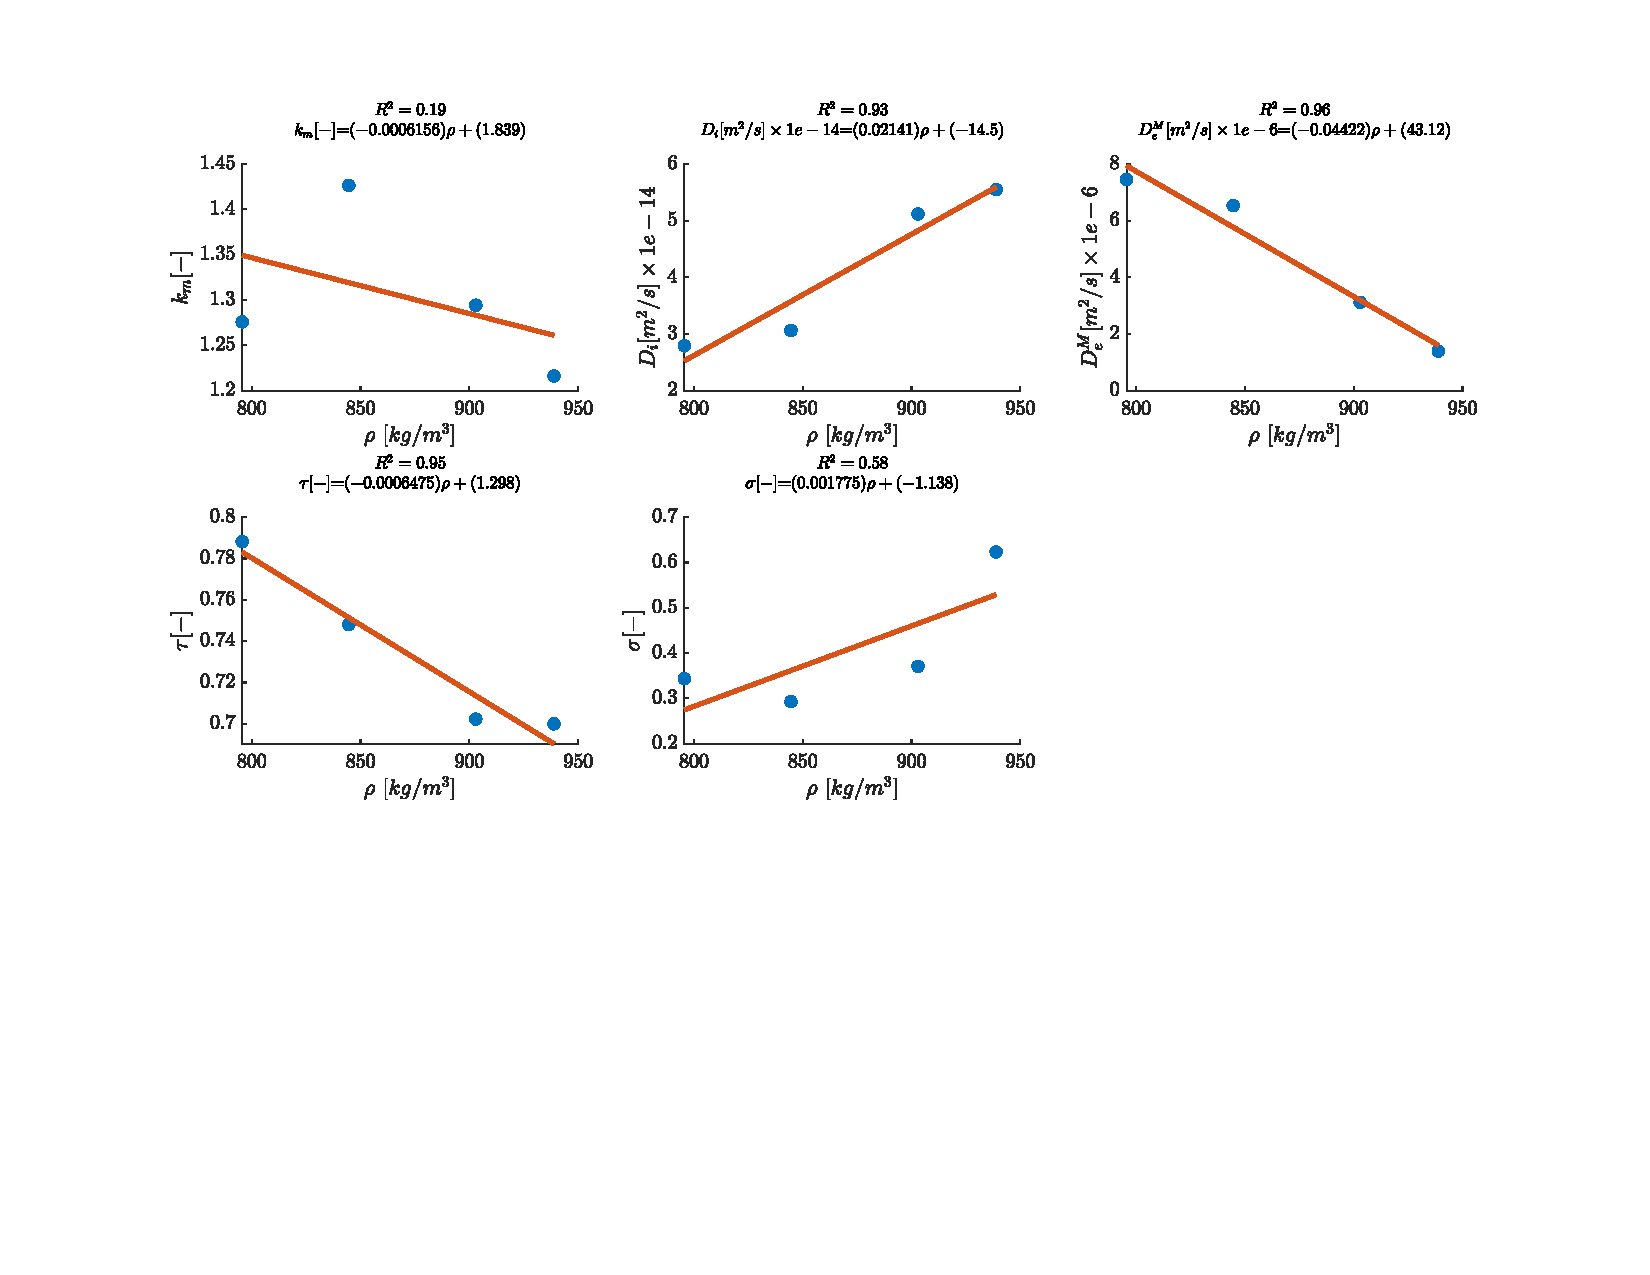
\includegraphics[trim = 3cm 8cm 17.7cm 7.7cm,clip,width=\columnwidth]{/Results_estimation/Trend_Lines_order_1.pdf}
			\caption{Dependency of ${\color{orange}\Upsilon}$}
			\label{fig: results_upsilon}
		\end{subfigure}
		\hfill
		\begin{subfigure}[b]{0.49\columnwidth}
			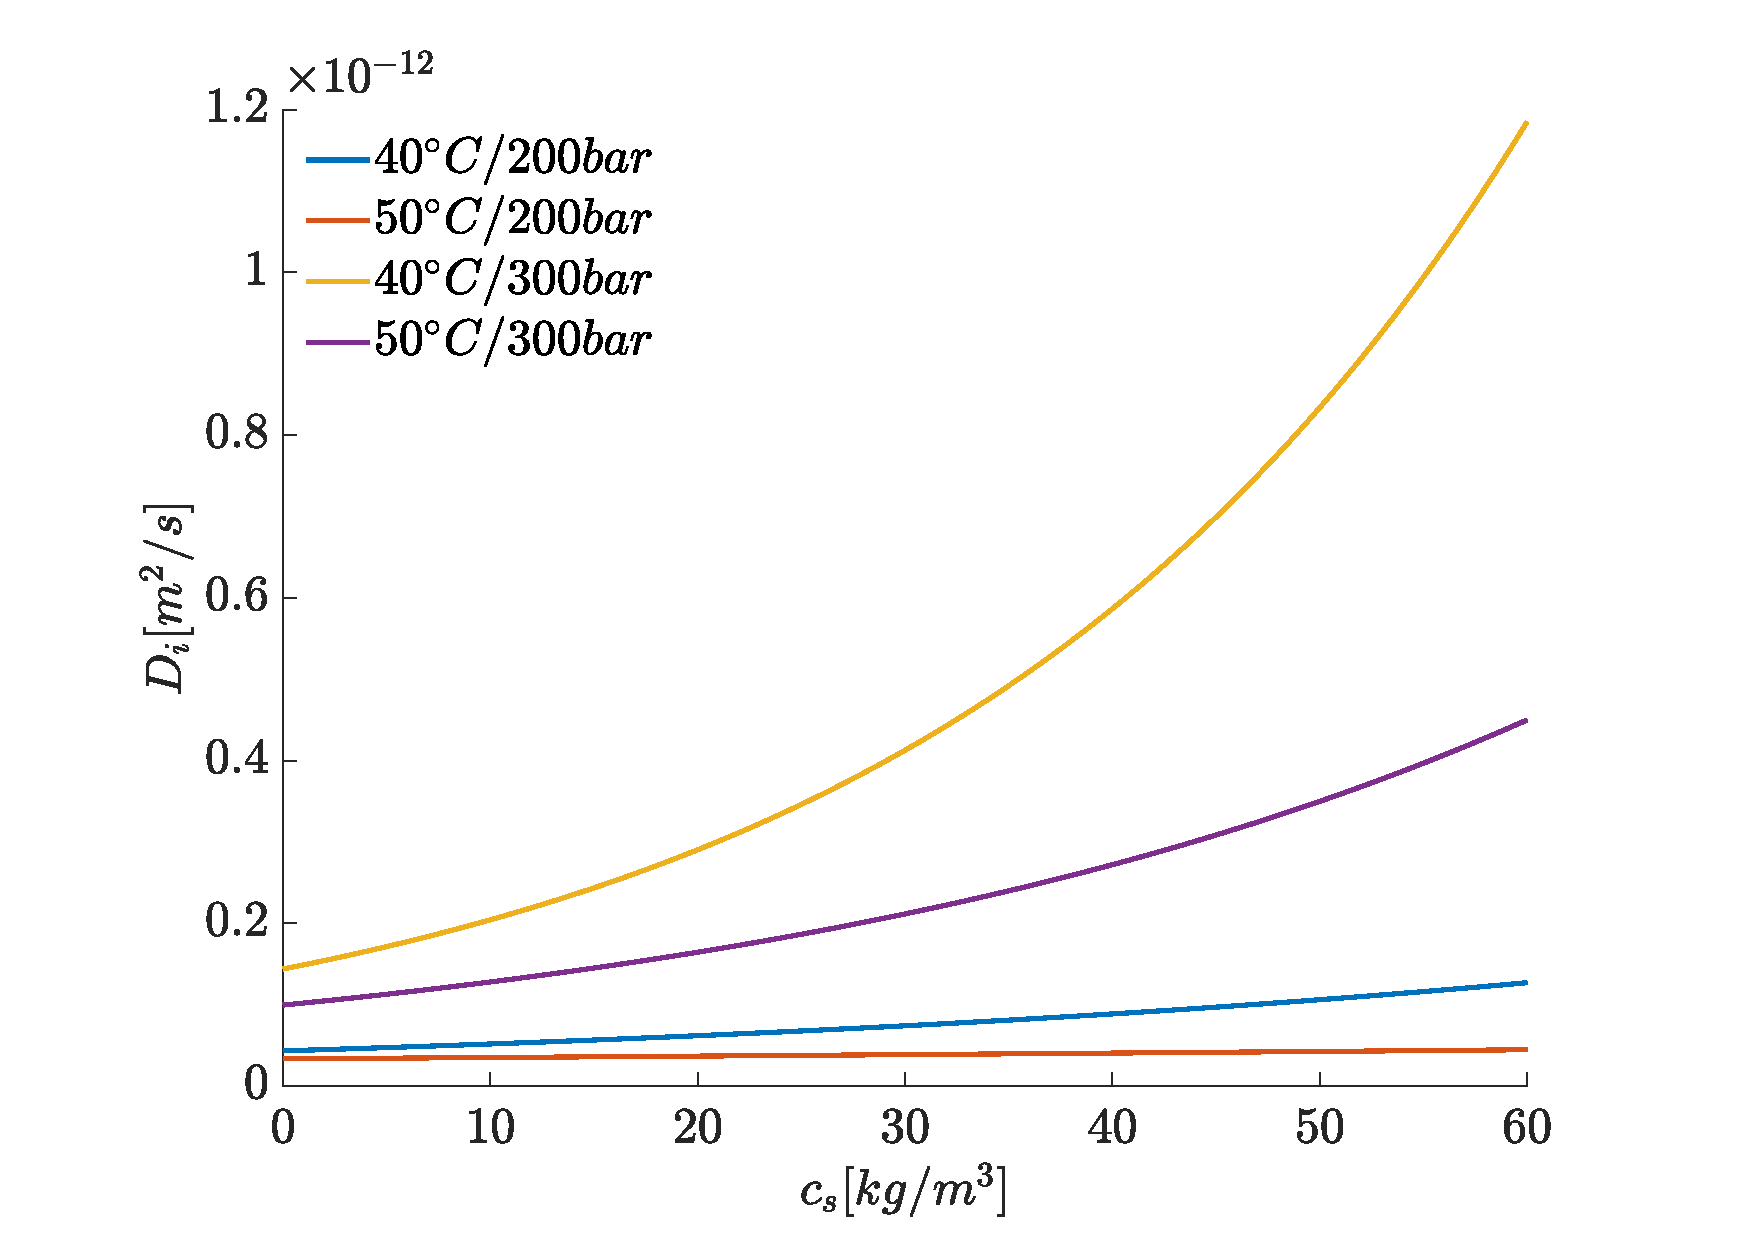
\includegraphics[trim = 1.0cm 0cm 3cm 0cm, clip, width=\columnwidth]{/Results_estimation/D_i_Uppsilon_results.pdf}
			\caption{Dependency of ${\color{orange}D^R_i}$}
			\label{fig:Di_upsilon_res}
		\end{subfigure}
		\begin{subfigure}[b]{0.49\columnwidth}
			\centering
			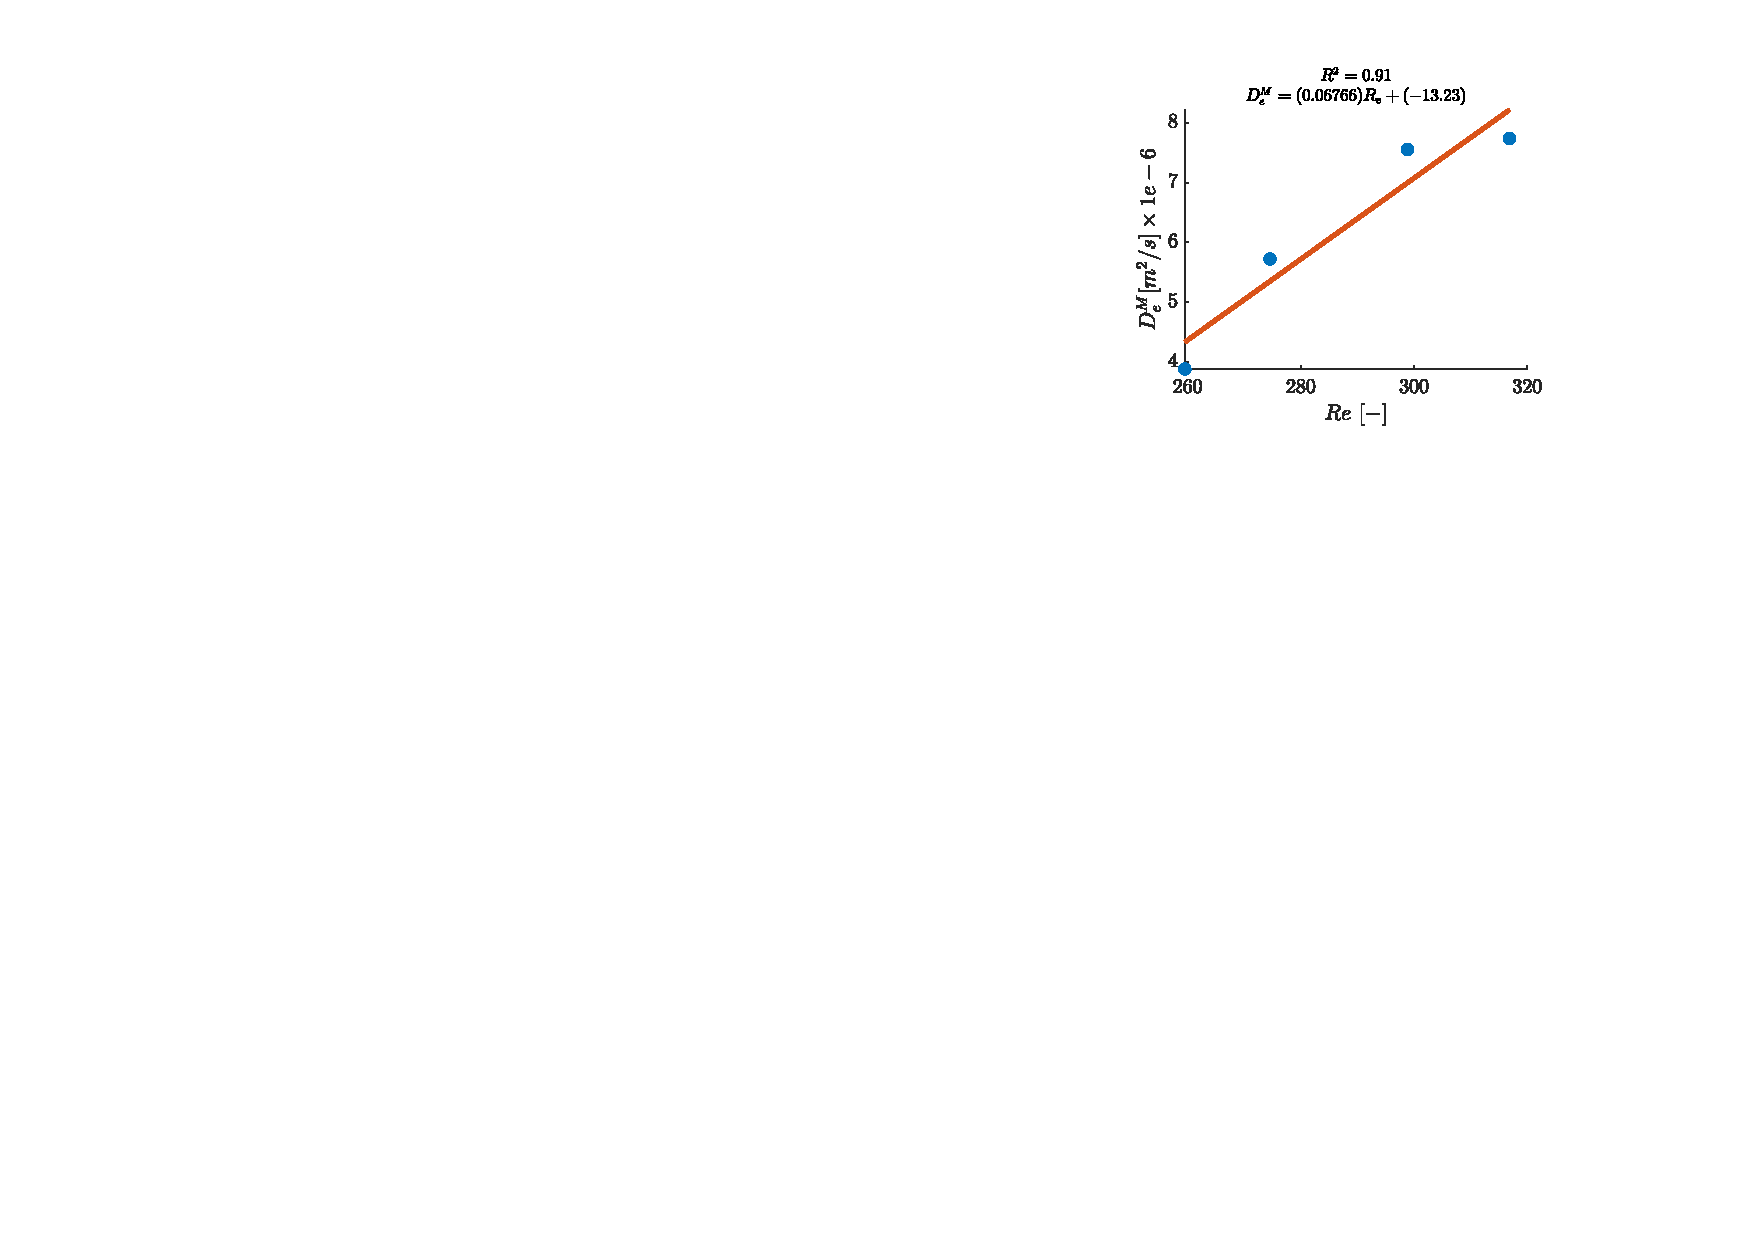
\includegraphics[trim = 19.0cm 13.8cm 3.5cm 1.0cm,clip,width=\columnwidth]{/Results_estimation/Trend_Lines_D_e.pdf}
			\caption{Dependency of ${\color{orange}D^M_e}$}
			\label{fig: results_De}
		\end{subfigure}
		\caption{Results of parameter estimation}
		\label{fig: estimation_results_DI_GAMMA}
	\end{figure}
	
	The axial diffusion coefficient obtained from the optimizer seems is relatively high if compared to the internal diffusion coefficients. The values of ${\color{orange}D_e^M}$ have similar order of magnitude as reported in literature( \citet{ReisVasco2000}). %The relatively high values of the axial diffusion coefficients might be justified by taking into account low values of flow rate used in all the experiments. 
	The axial diffusion can be further analysed by defining the Pecelt number (${\color{orange}P_e} = v \times {\color{magenta}d_p} / {\color{orange}D_e^M} $) and the Reynolds number (${\color{orange}R_e} = v \times {\color{magenta}d_p} / {\color{orange}\mu} $), where ${\color{magenta}d_p}=0.15~[m]$ is the characteristic dimension defined to be the extractor diameter and $\mu$ is the fluid viscosity. %The obtained Pecelt numbers have the order of magnitude of $1 \times 10^{8}$, which suggest that diffusion is negligible, and advection dominates mass transport. 
	The obtained Pecelt numbers are $P_e \gg 1$, which suggest that mass diffusion is negligible, and advection dominates mass transport. An idea to consider a relationship between the Peclet (indirectly the mass diffusion coefficient) and Reynolds numbers has been proposed by \citet{Chung1968}. 
	The Figure \ref{fig: results_De} shows that the obtained values of the mass diffusion coefficient increase almost linearly with increment of the Reynolds number.

	As the total amount of the oil present in the system is unknown, and as such it has been obtained from the optimizer. Given the dataset and the process model, the optimizer found that the best fit is obtained if the total mass of the oil reach a lower bound equal to 80 g. The lower bound was estimated by round up of the biggest value of collected cumulative amount of the extraction product. As the same raw material was used in all experiments, the same initial amount of solute is assumed for all the cases.
	
	The inital state estimation resulted in values of $\tau$ in range from 0.69 to 0.76. These values are relatively similar to each other. It can be concluded that in the used experimental set-up around 30\% of the solute was extracted to the fluid phase during the preparation period. 
	
	The noise present in each dataset is quantified by parameter $\sigma^2$. It can be observed dataset obtained at $40 ^\circ C$ / 200 bar and $30 ^\circ C$ / 300 bar have similar value of $\sigma^2\approx0.07$. The slightly better results were obtained for the experiment at $50 ^\circ C$ / 300 bar, when $\sigma^2\approx0.05$. The most noisy dataset corresponds to $50 ^\circ C$ / 200 bar, when $\sigma^2\approx0.12$. All values of $\sigma^2$ are relatively low, which suggest the mathematical model is capable to mimic the physical system up to the noise coming from the experiment.

	%The results obtained from the parameter estimation are used to develop a generalized process model. The model generalization is performed by introducing correlations which link the estimated parameters and the operating conditions. Since the experiments were performed under varying temperature and pressure, the influence of these variables is taken into account. To simplify the problem, the correlations are written as functions of fluid density rather than temperature and pressure. Since the optimizer found that ${\color{orange}k_m}$, $m_{total}$ and $C_{lim}$ don't change with the density variations, they are assumed to be constants and not considered further.
		
	
%	\begin{figure}[!h]
%		\centering
%		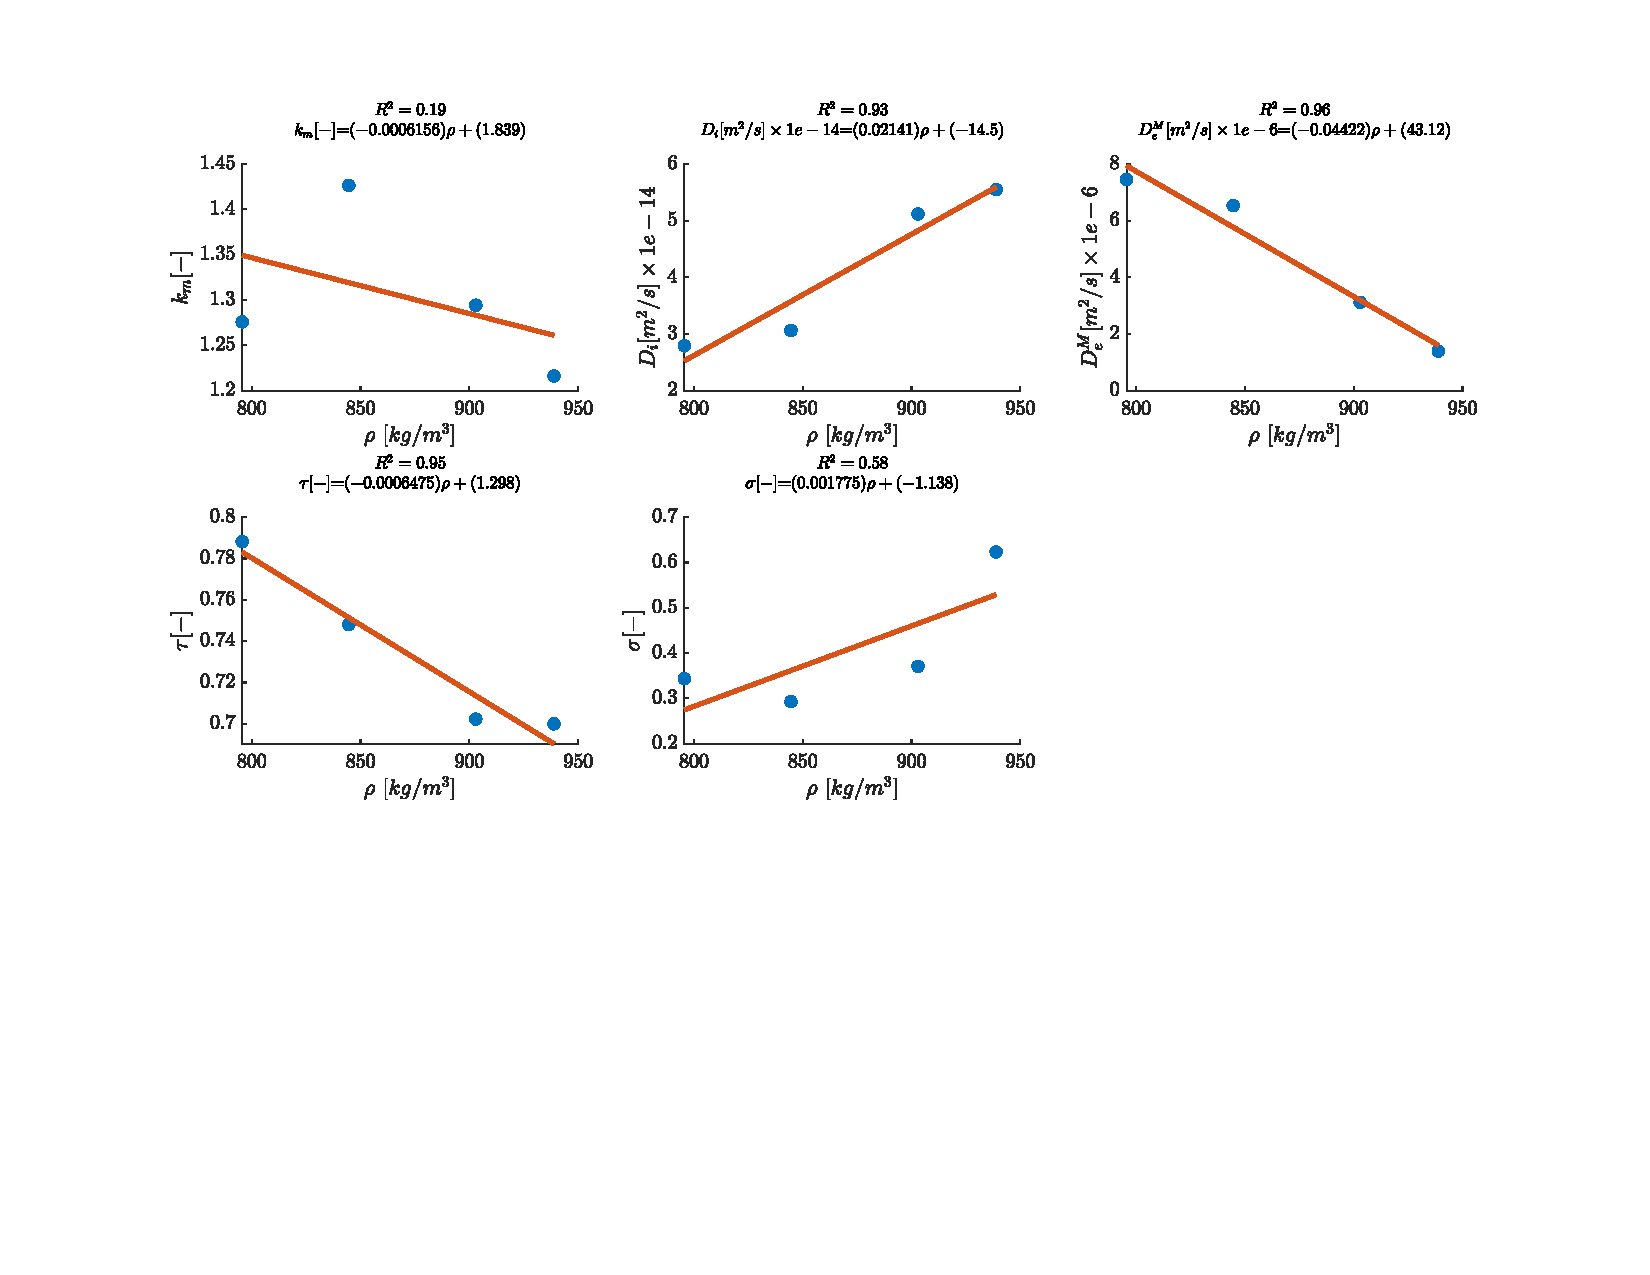
\includegraphics[trim = 11.7cm 14cm 2.3cm 1cm,clip,width=\textwidth]{/Results_estimation/Trend_Lines_order_1.pdf}
%		\caption{Second-order polynomial regression of fitted parameters (${\color{orange}D_i^R}$ and ${\color{orange}D_e^M}$) as a function of fluid density $\rho_f$}
%		\label{fig:Regression_2}
%	\end{figure}

	
	
\end{document}